\documentclass[12pt,letterpaper]{article}

\usepackage{amsmath, amsthm, amsfonts, amssymb}
\usepackage{graphicx,hyperref}
\usepackage{microtype, parskip}
\usepackage[comma,sort&compress]{natbib}
\usepackage{docmute}
\usepackage{subcaption, multirow, morefloats}
\usepackage{wrapfig, rotating}

\frenchspacing

\captionsetup[subfigure]{position = top, labelfont = bf, textfont = normalfont, singlelinecheck = off, justification = raggedright}

\begin{document}
\section{Methods}

\subsection{Species information}

\subsubsection{Informal phylogeny}

\subsection{Biogeographic network}

\begin{figure}[ht]
  \centering
  \begin{subfigure}[b]{0.4\textwidth}
    \caption{}
    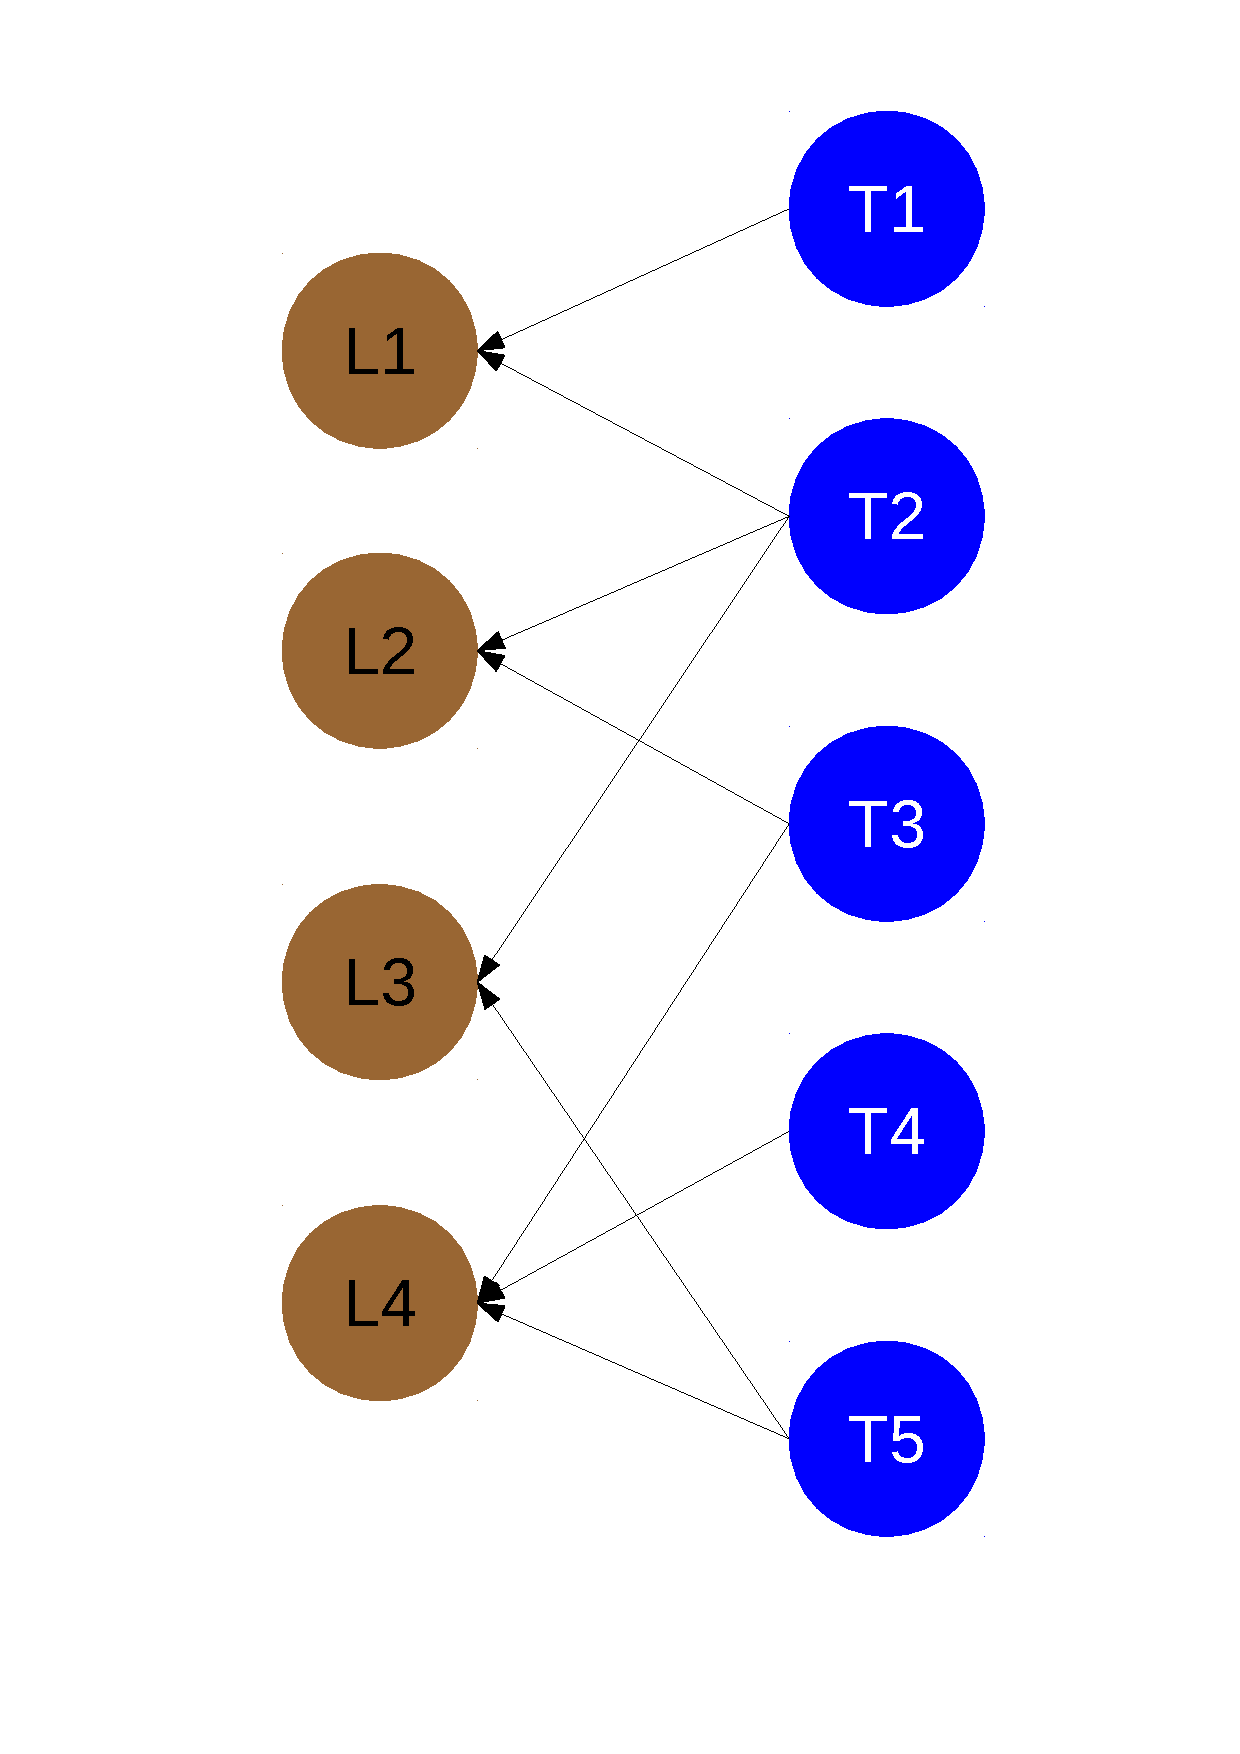
\includegraphics[height = 0.5\textheight, width = \textwidth, keepaspectratio = true]{figure/bipartite_graph}
    \label{subfig:bip_net}
  \end{subfigure}

  \begin{subfigure}[b]{0.4\textwidth}
    \caption{}
    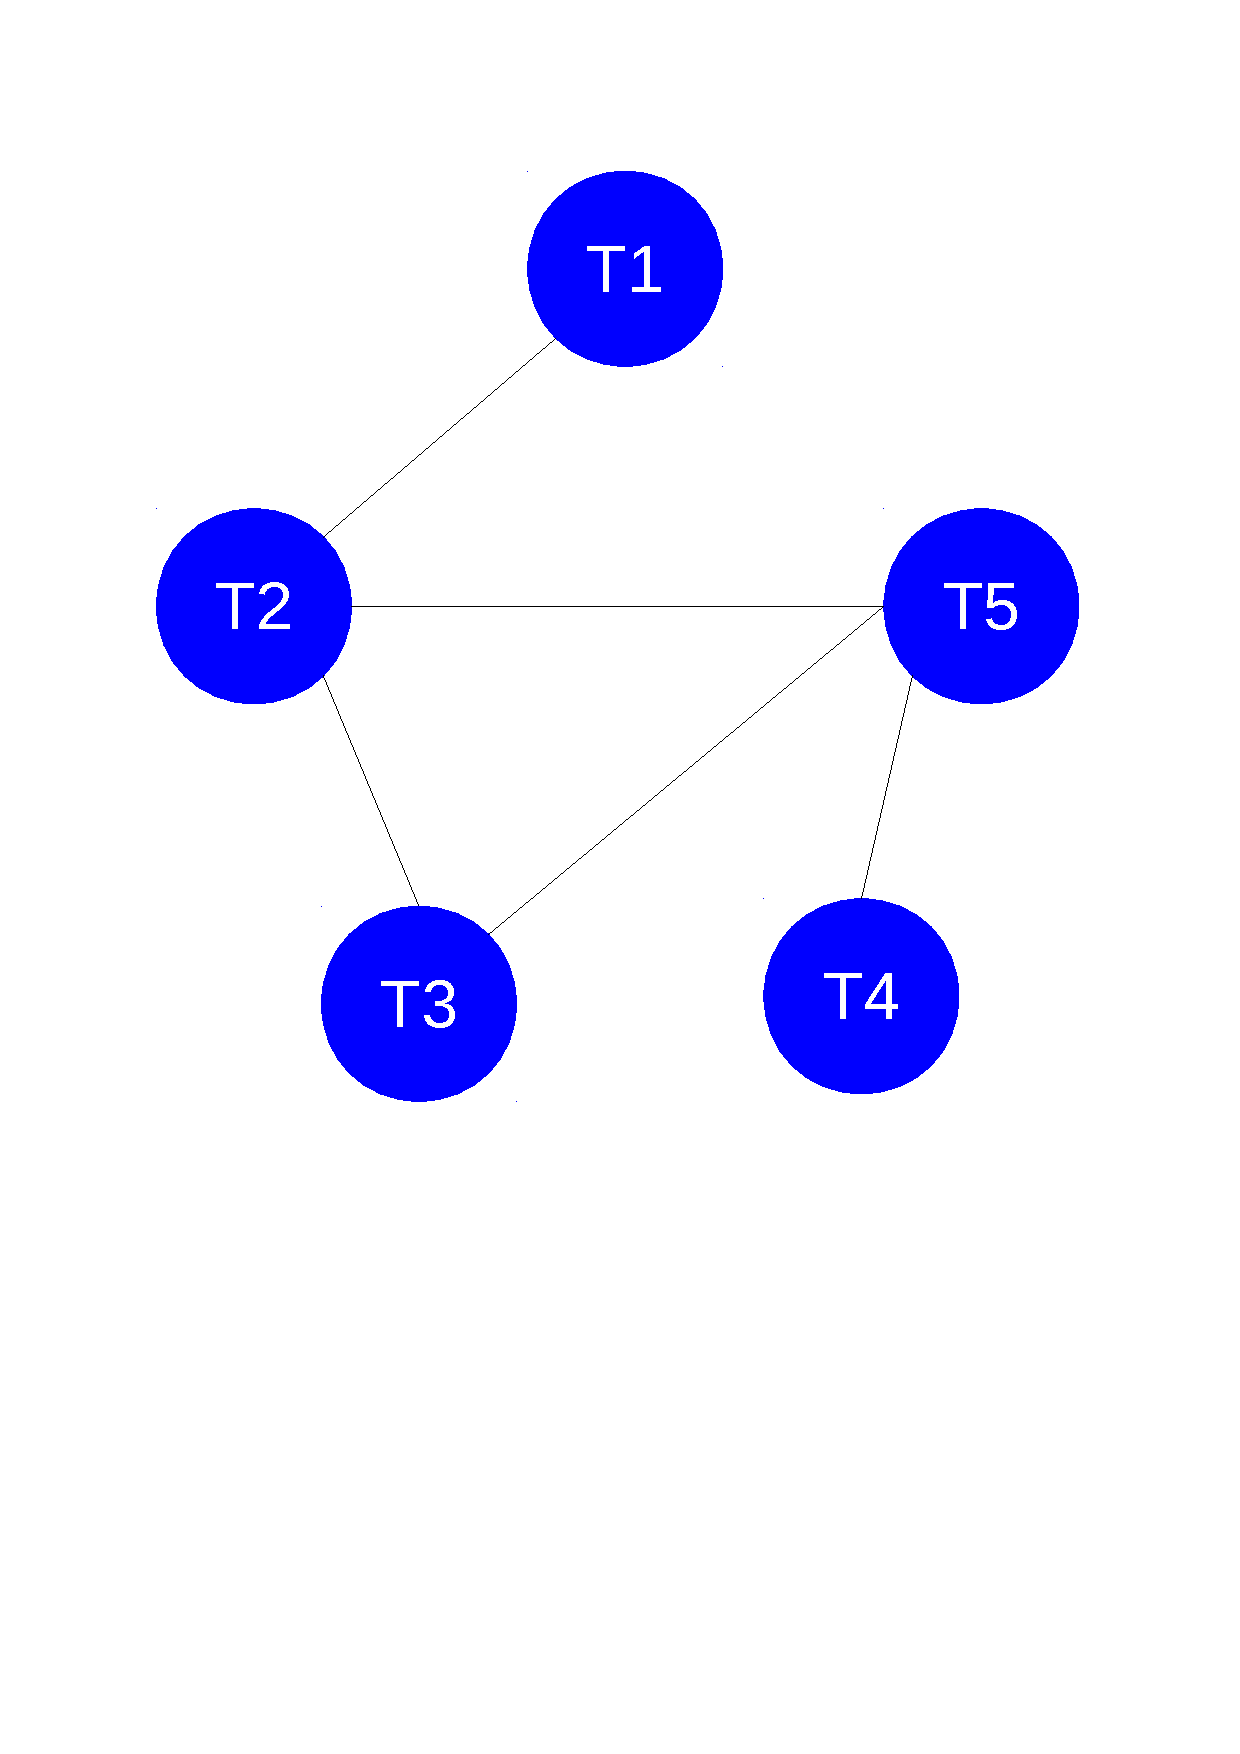
\includegraphics[height = 0.5\textheight, width = \textwidth, keepaspectratio = true]{figure/one_mode}
    \label{subfig:one_mode}
  \end{subfigure}
  \caption{Bipartite and one mode graphs.}
  \label{fig:graphs}
\end{figure}




\subsection{Co-occurrence model}

Poisson distribution with rate \(\lambda\) is defined 
\begin{align}
  \mathrm{Poisson}(n_{i} | \lambda_{i}) &= \frac{1}{n_{i}!} \lambda^{n_{i}} \exp(-\lambda_{i}) 
  \label{eq:pois} \\
  \lambda_{i} &= \exp(\beta^{T}\mathbf{X_{i}} + h_{i}).
  \label{eq:lambda}
\end{align}

Negative binomial distribution parameterized with mean \(\mu\) and overdispersion \(\phi\) is defined
\begin{align}
  \mathrm{Negative\ binomial}(y_{i} | \mu_{i}, \phi) &= {y_{i} + \phi -1 \choose y_{i}} \left(\frac{\mu_{i}}{\mu_{i} + \phi}\right)^{y_{i}} \left(\frac{\phi}{\mu_{i} + \phi}\right)^{\phi}
  \label{eq:neg_bin} \\
  \mu_{i} &= \exp(\beta^{T}\mathbf{X_{i}} + h_{i}) 
  \label{eq:mu} \\
  \phi &\sim \mathrm{halfCauchy}(2.5).
  \label{eq:phi} 
\end{align}

\(\mathbf{X}\) is defined as an \(n \times K\) matrix where \(n\) is the number of observations and \(K\) is the number of covariates of interest. As described above, the covariates of interest are the dietary and locomotor categories of a species and its body mass. While body mass is a continuous covariate, dietary and locomotor categories are index variables that need to be transformed into multiple binary covariates or indicator variables. To do this, for each of these variables were each transformed into \(n \times (k - 1)\) matrices where \(k - 1\) is the number of categories of the index variable (3 and 4, respectively). Only \(k - 1\) indicator variables are necessary as the intercept takes on the remaining category. Finally, a column of 1-s in included in the matrix \(\mathbf{X}\) whose corresponding \(\beta\) coefficient is the intercept. In total, \(K\) equals 7.
% Do I want to change locomotor and dietary categories into random effects? Might improve interpretability.

For the parameterizations of the means for both the Poisson (Eq. \ref{eq:lambda}) and negative binomial models (Eq. \ref{eq:mu}), a unique coefficient \(\beta\) is assigned to each of the covariates and are given a diffuse, weakly informative prior (\(\beta_{k} \sim \mathcal{N}(0, 10)\)).

\(h\), or phylogenetic effect, is defined as a random multivariate normally distributed variable whose covariance matrix known up to a constant \(\sigma_{p}\) (Eq. \ref{eq:phy_sim}).
\begin{align}
  h &\sim \mathrm{Multivariate\ }\mathcal{N}(0, \mathbf{\Sigma}) \label{eq:phy_sim} \\
  \mathbf{\Sigma} &= \sigma_{p}^{2} \mathbf{V}_{phy} \nonumber \\
  \sigma_{p} &\sim \mathrm{halfCauchy}(2.5). \nonumber
\end{align}

The overdispersion parameter \(\phi\) of the negative binomial distribution was given weakly informative half-Cauchy prior distribution (Eq. \ref{eq:phi}).

Graphical summaries of the Poisson and negative binomial models, along with all values for the prior distributions, are presented in Figures \ref{fig:poismod_diagram} and \ref{fig:nbinmod_diagram}, respectively.
\begin{figure}[ht]
  \centering
  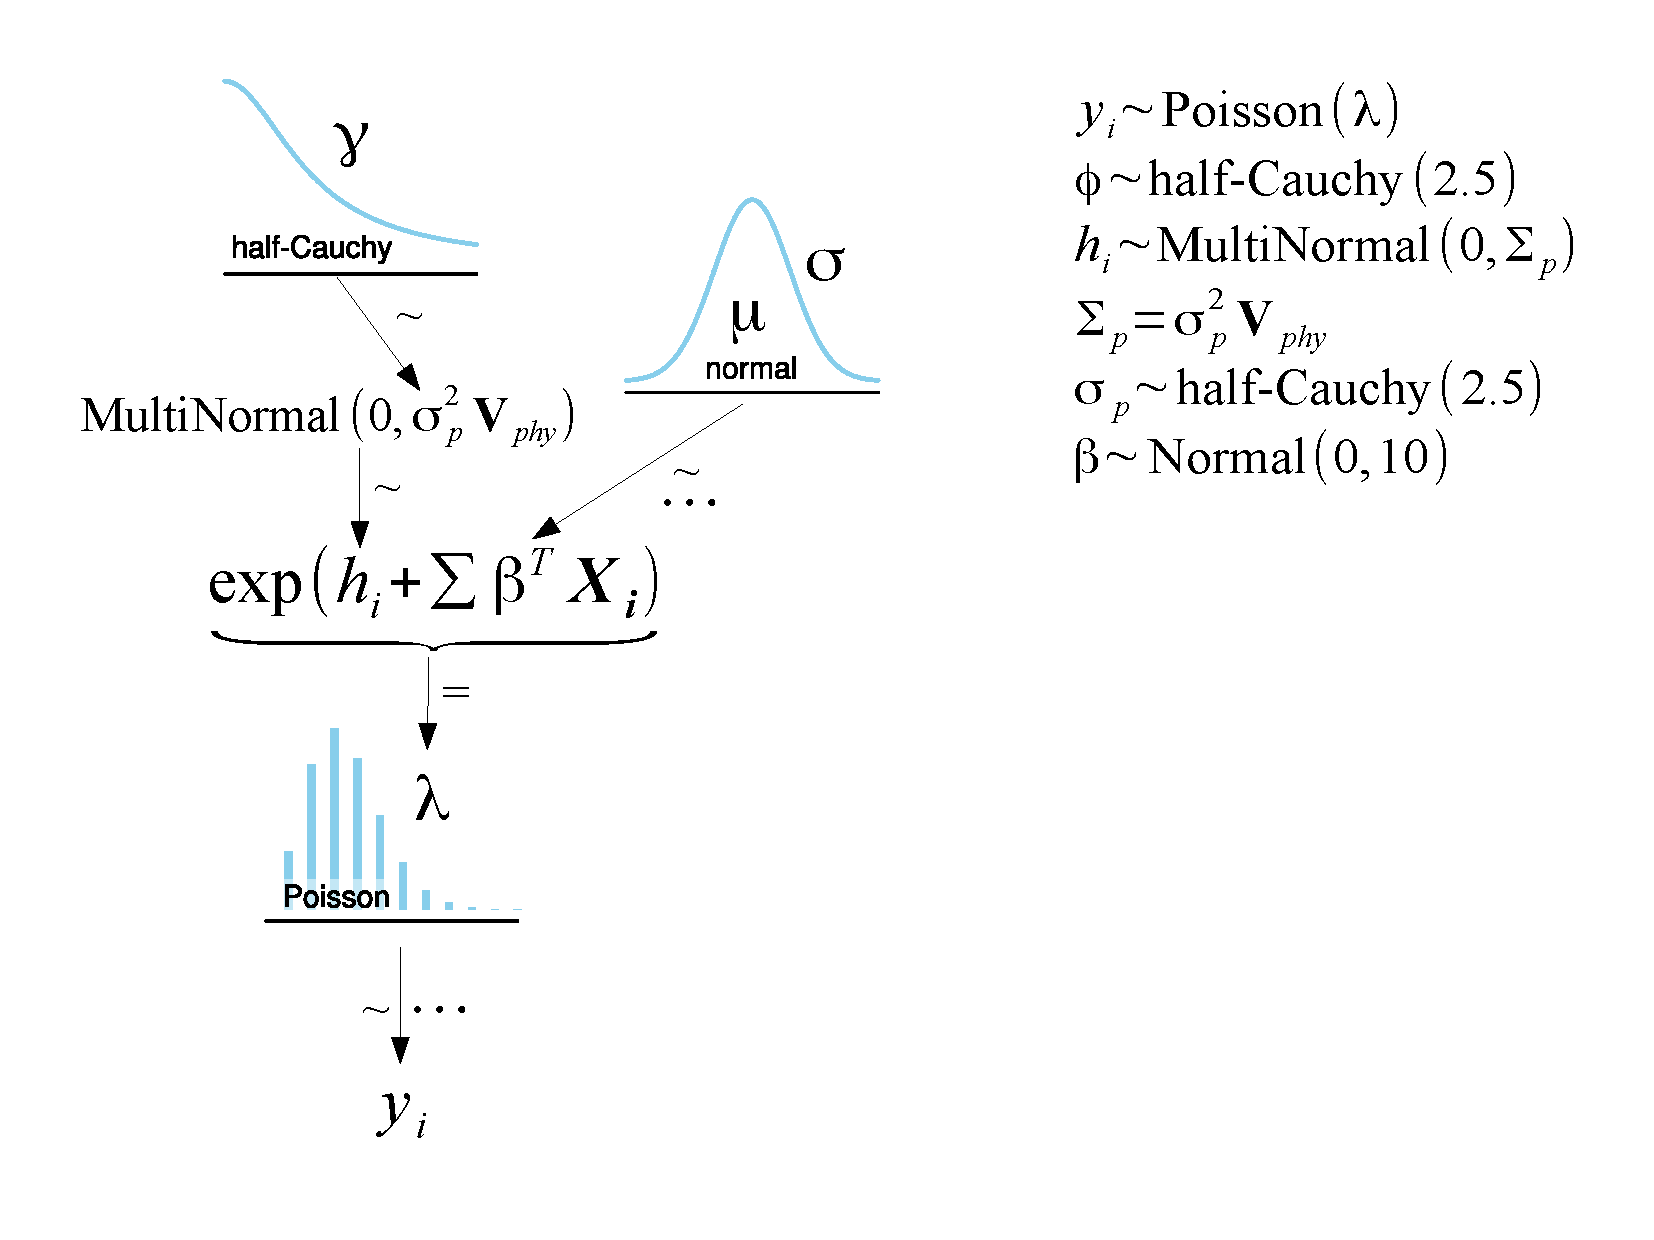
\includegraphics[height = 0.5\textheight, width = \textwidth, keepaspectratio = true]{figure/mammal_degree_model}
  \caption{Poisson model}
  \label{fig:poismod_diagram}
\end{figure}

\begin{figure}[ht]
  \centering
  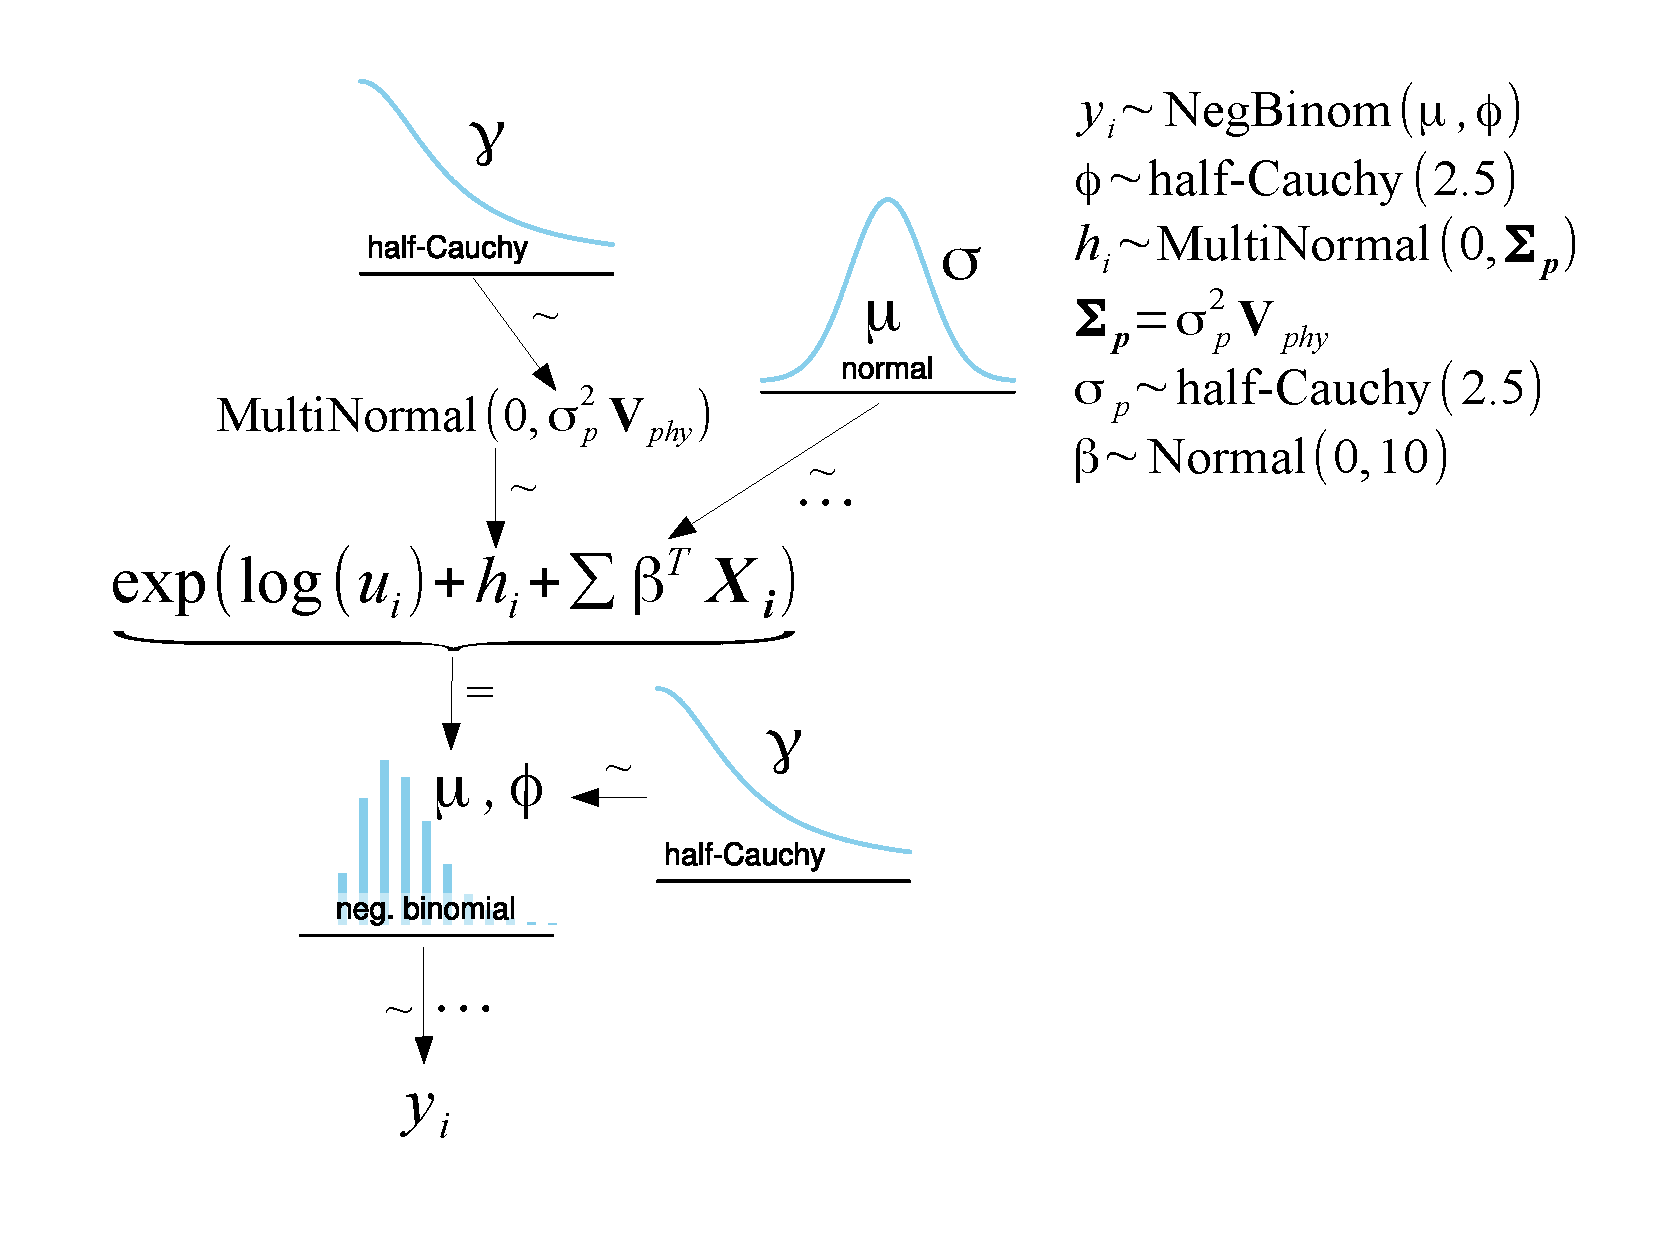
\includegraphics[height = 0.5\textheight, width = \textwidth, keepaspectratio = true]{figure/mammal_deg_over_model}
  \caption{Negative binomial model}
  \label{fig:nbinmod_diagram}
\end{figure}

\subsection{Posterior predictive checks}

A models utility in making predictive and descriptive statements is dependent on its fit to the data and the questions of interest.


\subsection{Predictive power}

\begin{figure}[ht]
  \centering
  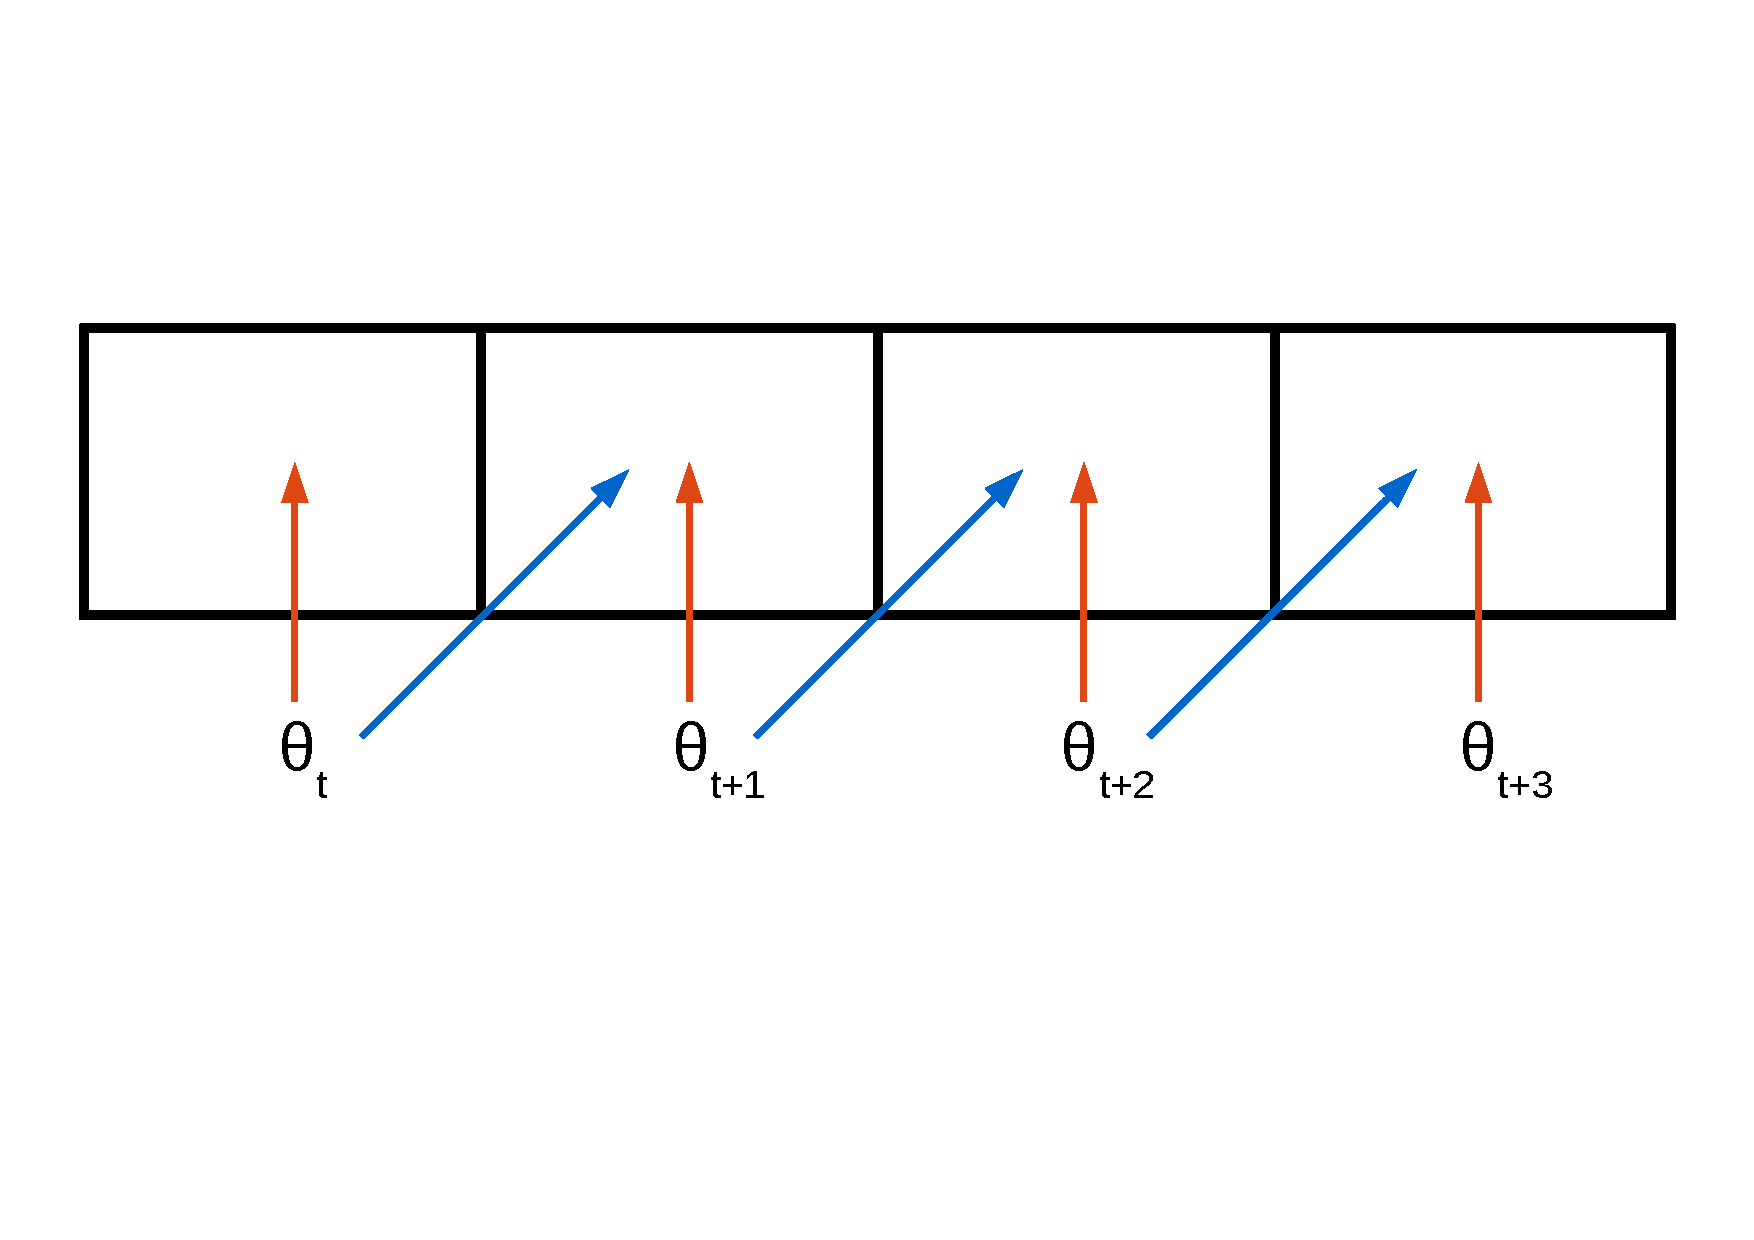
\includegraphics[height = 0.5\textheight, width = \textwidth, keepaspectratio = true]{figure/predict_perform}
  \caption{CAPTION}
  \label{fig:concept}
\end{figure}


\end{document}
